\section{Simulation Results}\label{sec:results}

\begin{table}[t]\small
    \centering
    \caption{Details of the benchmarks used in this paper.}
      \begin{tabular}{|c|c|c|c|c|c|l|}\hline

      Benchmark     & $|O|$ & $n_i$    & $n_o$    & $D_p$     &$D_e$ \\\hline\hline
      RA100         & 100   & 6	       & 6	      &16	           &5 mixers       \\\hline
      RA70          & 70    & 7    & 8  & 10      &3 mixers, 2 detectors       \\\hline
      CPA           & 55    & 7    & 8  & 9       &3 mixers, 2 detectors  \\\hline
      RA30          & 30    & 11     & 1   & 7   & 3 mixers, 1 detector, 1 filter  \\\hline
      IVD           & 12    & 6     & 6   & 3    & 3 mixers, 2 detectors \\\hline
      PCR           & 7     & 4     & 1   & 3    & 2 mixers\\\hline
      \end{tabular}%
 %     \caption*{RA100, RA70 and RA30 are randomly generated assays.}\footnotesize
    \label{tb_input_graph}%
  \end{table}%


\begin{table*}[t] 
\footnotesize
\centering
\renewcommand{\tabcolsep}{7.35pt}
\renewcommand{\arraystretch}{1}
\caption{Results of Test Pattern Generation with Single Pressure Source and Single Pressure Sensor}
\label{tb_test}
\begin{tabular}{cr r ccccccc r ccccccc} \hlinewd{0.7pt}
\multicolumn{2}{c}{FPVA} &
\multicolumn{1}{c}{} &
\multicolumn{7}{c}{Direct Approach} &
\multicolumn{1}{c}{} &
\multicolumn{7}{c}{Loop Acceleration} \\
\cline {1-2}\cline {4-10}\cline {12-18} 
\multicolumn{1}{c}{Dimension} &
\multicolumn{1}{c}{$n_v$} &
\multicolumn{1}{c}{} &
\multicolumn{1}{c}{$n^d_p$} &
\multicolumn{1}{c}{$t^d_p(s)$} &
\multicolumn{1}{c}{$n^d_c$} &
\multicolumn{1}{c}{$t^d_c(s)$} &
\multicolumn{1}{c}{$n^d_l$} &
\multicolumn{1}{c}{$t^d_l(s)$} &
\multicolumn{1}{c}{$N^d$} &
% \multicolumn{1}{c}{$T^d(s)$} &
\multicolumn{1}{c}{} &
\multicolumn{1}{c}{$n^a_p$} &
\multicolumn{1}{c}{$t^a_p(s)$} &
\multicolumn{1}{c}{$n^a_c$} &
\multicolumn{1}{c}{$t^a_c(s)$} &
\multicolumn{1}{c}{$n^a_l$} &
\multicolumn{1}{c}{$t^a_l(s)$} &
\multicolumn{1}{c}{$N^a$} \\
% \multicolumn{1}{c}{$T^a(s)$} \\


\hlinewd{0.6pt}

5 $\times$5 &40&&2	&0.02	&8	&0.67	&3	&0.01	&13	&&2	&0.02	&8	&0.16	&3	&0.02	&13	\\
10$\times$10&380&&2	&0.72	&18	&46	&3	&0.04	&23	&&2	&2.61	&18	&12	&3	&0.03	&23	\\
15$\times$15&420&&2	&48	&28	&984	&4	&0.12	&34	&&2
	    &78	&28	&40	&3      &73	&33	   	\\
20$\times$20&760&&2	&758	&*	&*	&*	&*	&*	&&2	&363	&38	&146	&3	&163	&43	\\
25$\times$25&1200&&*	&*	&*	&*	&*	&*	&*	&&3	&1200	&48	&472	&3	&966	&54	\\
30$\times$30&1740&&*	&*	&*	&*	&*	&*	&*	&&3	&1201	&58	&1648	&4	&1243	&65	\\

% 5  $\times$ 5   &39  &&1 $\times$  1&5 $\times$ 5  &&5  & 0.3  &&8  &0.2 & &  4  &  2   &&17 & 2.5 \\ 
% 10 $\times$ 10  &176 &&2 $\times$  2&5 $\times$ 5  &&4  & 4    &&18 &5   & &  4  &  10  &&26 & 19  \\
% 15 $\times$ 15  &411 &&3 $\times$  3&5 $\times$ 5  &&8  & 17   &&28 &26  & &  8  &  127 &&44 & 170 \\
% 20 $\times$ 20  &744 &&4 $\times$  4&5 $\times$ 5  &&16 & 35   &&38 &41  & & 16  & 742  &&70 & 818 \\
% 30 $\times$ 30  &1704&&6 $\times$  6&5 $\times$ 5  &&20 & 255  &&58 &171 & & 20  & 1492 &&98 & 1918\\
\hlinewd{0.7pt}
\multicolumn{18}{l}{* -- No valid result}\\
\end{tabular}
\end{table*}





The proposed method was implemented in C++ and tested on a PC with \SI[mode=text]{3.20}{\GHz} CPU and
\SI{8}{GB} memory. We demonstrate the results using three real-life assays and three randomly generated assays. The information of these test cases is shown in Table~\ref{tb_input_graph}, where CPA (Colorimetric Protein Assay), IVD (In-Vitro Diagnostics) and PCR (Polymerase Chain Reaction) are real-world assays \textcolor{red}{\cite{pop2016microfluidic}} and the other three assays are randomly generated. The Column $\boldsymbol{|O|}$ in Table~\ref{tb_input_graph} shows the number of operations in each assay. The Columns $\boldsymbol{n_i}$ and $\boldsymbol{n_o}$ are the number of inputs and outputs of each assay, respectively. The Column $\boldsymbol{D_p}$ gives the depth of the sequencing graph corresponding to each assay. The Column $\boldsymbol{D_e}$ lists the number of available devices for each assay, respectively. \textcolor{red}{The execution latencies of mixing, detection, and filtration operations are set to 4 s, 7 s, and 3 s in the benchmarks, respectively \cite{pop2016microfluidic}.} Moreover, in the experiments, we used Gurobi \cite{gurobi} to solve the optimization problems.

\subsection{\textcolor{red}{Synthesis Results of the Proposed Design Flow}}

\textcolor{red}{In this part, we first report the synthesis results of each stage in the proposed design flow in Table~\ref{tb_test}, including scheduling, architectural synthesis, as well as flow-path planning.}

The result of scheduling with storage minimization is shown in the columns $\boldsymbol{c_t}$, $\boldsymbol{t^E}$ and $\boldsymbol{t_s}$, where \textcolor{red}{$\boldsymbol{c_t}$ is the total amount of time that fluids are stored,} $\boldsymbol{t^E}$ is the execution time of the assay defined in (\ref{eq:latest_finishing}), and $\boldsymbol{t_s}$ is the runtime for solving the optimization problem (\ref{eq:minobj})--(\ref{eq:op_cond}), which was limited to 30 minutes for the solver to return the best-effort results. It can be seen that the execution of each bioassay is completed within a reasonable time.

In architectural synthesis, we use a connection grid to determine device locations and channel segments connecting them. The size of the grid is shown in column $\boldsymbol{G}$. Moreover, \textcolor{red}{the numbers of
channel segments} and valves in the chip are shown in the columns $\boldsymbol{n_e}$ and $\boldsymbol{n_v}$, respectively. Note the valves counted in the experiments do not include those used in mixers. The runtimes to generate chip architectures are shown in the column $\boldsymbol{t_r}$.
\textcolor{red}{Moreover, with the generated chip architecture, we re-perform the proposed scheduling method to map the bioassay onto the synthesized architecture, thus generating an updated scheduling with accurate transportation latencies. Correspondingly, the updated execution times of assays are shown in the column $\boldsymbol{t^{Eu}}$.}

%After completing the architectural synthesis, transportation tasks specified in the scheduling are mapped to the chip, so that certain flow paths can be constructed to realize the transportation network without any conflict.
% During the flow-path planning, the total number of transportation-task groups generated after performing the sweepline algorithm is shown in the column $\boldsymbol{n_g}$. Inside each group, when mapping the transportation tasks to the biochip, their corresponding flow paths may conflict with each other, leading to a conflicting group. Accordingly, the number of conflicting transportation-task groups is shown in the column $\boldsymbol{n_{cg}}$. We can see that transportation conflicts exists in most groups and all these conflicts are eliminated successfully after implementing the proposed adjustment strategies.

After flow-path planning, the total number of valves in the chip is reported in the column $\boldsymbol{n_{tv}}$.
\textcolor{red}{It can be seen that new valves are introduced into the chip. We analyze this for two reasons: 1) since pumps and waste ports are added to the chip in this stage, these devices should be connected to the previously allocated devices such as mixers by constructing new flow channels. These channels may intersect with previously constructed flow paths, thereby leading to some extra valves and 2) the number of pumps and waste ports introduced to the chip is minimized to reduce extra chip cost (see columns $\boldsymbol{n_p}$ and $\boldsymbol{n_w}$), thus increasing the number of new constructed channels.}
The numbers of crossings and T-junctions in the final chip architecture are shown in the columns $\boldsymbol{n_{cr}}$ and $\boldsymbol{n_{tj}}$, respectively.

Moreover, the total length of flow channels in the final chip is reported in the column $\boldsymbol{l_n}$.
% Moreover, the number of deadlocks is shown in the column $\boldsymbol{d_{k}}$, and all of them are eliminated by solving the ILP model defined in Section~\ref{sec:res_storage_deadlock}.
The final execution time of the assay is shown in the column $\boldsymbol{t^{E'}}$, which is a little bit longer than the one shown in the column $\boldsymbol{t^{Eu}}$ due to the effects of the proposed scheduling adjustment method. Finally, the runtimes of the flow-path planning are shown in the column $\boldsymbol{t_p}$, which are acceptable for a high-quality transportation network without any conflict.


\begin{figure}[t]
    \centering
    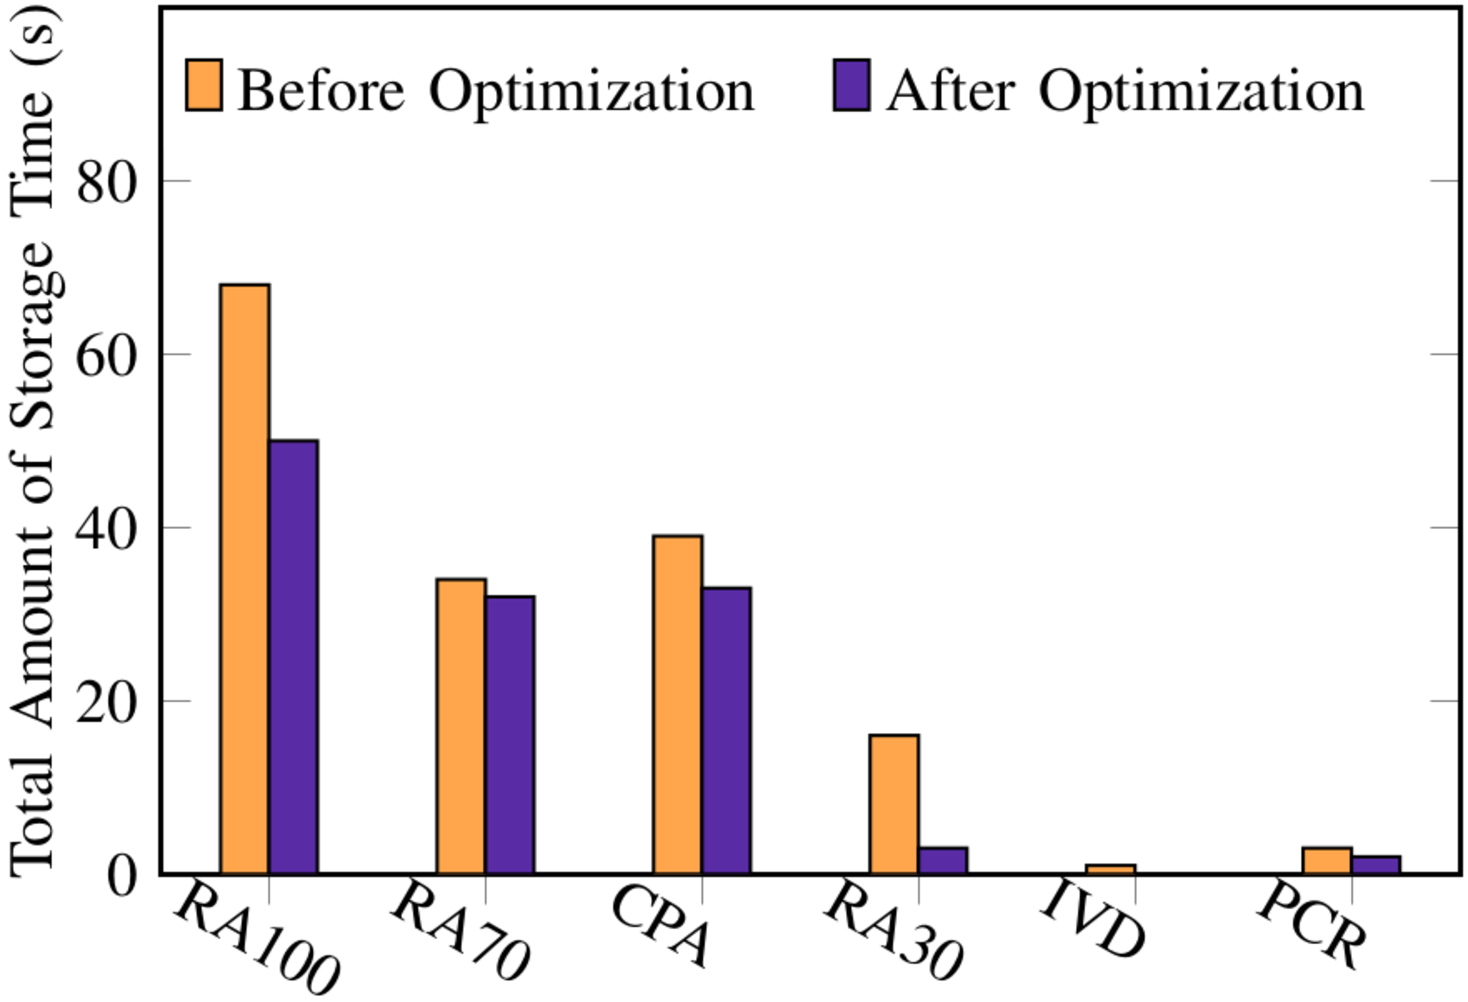
\includegraphics[width=0.85\linewidth]{Visio/storage_cmp.pdf}
  \caption{\textcolor{red}{Comparison of the total amount of time that fluids are stored before and after applying the proposed storage optimization method.}}
      \label{fig:storage_cmp}
%\vspace{-0.5cm}
\end{figure}



\pgfplotsset{compat=1.3,
    /pgfplots/ybar legend/.style={
    /pgfplots/legend image code/.code={%
       \draw[##1,/tikz/.cd,yshift=-0.25em]
        (0cm,0cm) rectangle (5pt,0.8em);},
   }
}

\subsection{\textcolor{red}{Performance Validation of the Proposed Optimization Methods}}

\textcolor{red}{In this subsection, the performance of several optimization methods in the proposed synthesis flow is validated in detail.}

We first evaluate the effectiveness of the proposed storage optimization method in scheduling. \figname~\ref{fig:storage_cmp} shows the comparison results on \textcolor{red}{the total amount of time that fluids are stored before and after incorporating this method into the scheduling.} It can be seen that \textcolor{red}{the total amount of time that fluids are stored} in each assay is reduced significantly after applying the proposed optimization method.  Moreover, \figname~\ref{fig:ideal_cmp} shows the comparison of execution time of assays, the number of \textcolor{red}{routing channels}, and the number of valves in the two cases with and without considering storage optimization.
It can be observed that storage optimization generated comparable execution time in the cases IVD and PCR, but the execution time of RA30 is slightly increased, which is acceptable for most biochemical experiments. However, the numbers of \textcolor{red}{routing channels} and valves in the result of RA30 are much smaller, \textcolor{red}{because storage optimization is partially achieved by reducing the number of fluid-storage operations, thus reducing the numbers of routing channels and valves that need to be constructed during architectural synthesis.}
\begin{figure}[t]
{\figurefontsize
\centering
\input{Fig/ideal_cmp.pdf_tex}
\caption{\textcolor{red}{Comparison results in terms of the execution time of assay and the numbers of routing channels and valves before and after applying the proposed storage optimization method.}}
\label{fig:ideal_cmp}
}
\end{figure}
%improves the efficiency of channels and thus valves effectively so that fewer resources are required to execute the assays.

\begin{figure}[t]
{\figurefontsize
\centering
\vskip 5pt
\begin{tikzpicture}
\begin{axis}[
x=1.1cm, y=0.27cm, ymax=12, line width=0.75pt,
ylabel={Channel (Valve) Ratio}, ylabel shift=-6pt, 
xtick={1,...,6},xticklabels={RA100, RA70, CPA, RA30, IVD, PCR},
x tick label style={rotate=330, xshift=-15pt,yshift=-5pt,anchor=west}, 
xticklabel pos=left, xtick align=outside, xtick pos=left,
ytickmin=0,ytickmax=10, 
ytick={0,5,10}, yticklabels={0,0.5,1},
legend columns=2, legend style={at={(0.5,0.9)}, anchor=center, nodes={inner xsep=2pt},
draw=none, column sep=1pt},
ybar=0pt, bar width=7
]
   \addplot[line width=0.5pt, black, fill=orange!70!white] table[x=cir,y=edge] 
{edge_valve_percentage.dat};
   \addplot[line width=0.5pt, black, fill=blue!65!orange] table[x=cir,y=valve] 
{edge_valve_percentage.dat};

   \legend{Channel\hspace*{8pt}, Valve\hspace*{8pt}}
\end{axis}
\end{tikzpicture}

%\begin{tikzpicture}
\begin{axis}[
x=1.1cm, y=0.27cm, ymax=12, line width=0.75pt,
ylabel={Channel (Valve) Ratio}, ylabel shift=-6pt, 
xtick={1,...,6},xticklabels={RA100, RA70, CPA, RA30, IVD, PCR},
x tick label style={rotate=330, xshift=-15pt,yshift=-5pt,anchor=west}, 
xticklabel pos=left, xtick align=outside, xtick pos=left,
ytickmin=0,ytickmax=10, 
ytick={0,5,10}, yticklabels={0,0.5,1},
legend columns=2, legend style={at={(0.5,0.9)}, anchor=center, nodes={inner xsep=2pt},
draw=none, column sep=1pt},
ybar=0pt, bar width=7
]
   \addplot[line width=0.5pt, black, fill=orange!70!white] table[x=cir,y=edge] 
{edge_valve_percentage.dat};
   \addplot[line width=0.5pt, black, fill=blue!65!orange] table[x=cir,y=valve] 
{edge_valve_percentage.dat};

   \legend{Channel\hspace*{8pt}, Valve\hspace*{8pt}}
\end{axis}
\end{tikzpicture}

\caption{
\textcolor{red}{Channel and valve ratios with respect to the results of
architectural synthesis and the original channels and valves
in the connection grid.}}
\label{fig:edge_valve_percentage}
}
\end{figure}

 \begin{figure}[t]
 {\figurefontsize
 \centering
 \begin{tikzpicture}
\begin{axis}[
x=1.1cm, y=0.26cm, ymax=12, line width=0.75pt,
ylabel={Exec./Valve Ratio}, ylabel shift=-6pt, 
xtick={1,...,6},xticklabels={RA100, RA70, CPA, RA30, IVD, PCR},
x tick label style={rotate=330, xshift=-15pt,yshift=-5pt,anchor=west}, 
xticklabel pos=left, xtick align=outside, xtick pos=left,
ytickmin=0,ytickmax=10, 
ytick={0,5,10}, yticklabels={0,0.5,1},
legend columns=2, legend style={at={(0.5,0.9)}, anchor=center, nodes={inner xsep=2pt},
draw=none, column sep=1pt},
ybar=0pt, bar width=7
]
   \addplot[line width=0.5pt, black, fill=orange!70!white]
table[x=cir,y=exetime] 
{exe_time_valve_cmp.dat};
   \addplot[line width=0.5pt, black, fill=blue!65!orange] table[x=cir,y=valve] 
{exe_time_valve_cmp.dat};
   \legend{Execution Time\hspace*{9pt}, Valve\hspace*{8pt}}
\end{axis}
\end{tikzpicture}

% \begin{tikzpicture}
\begin{axis}[
x=1.1cm, y=0.26cm, ymax=12, line width=0.75pt,
ylabel={Exec./Valve Ratio}, ylabel shift=-6pt, 
xtick={1,...,6},xticklabels={RA100, RA70, CPA, RA30, IVD, PCR},
x tick label style={rotate=330, xshift=-15pt,yshift=-5pt,anchor=west}, 
xticklabel pos=left, xtick align=outside, xtick pos=left,
ytickmin=0,ytickmax=10, 
ytick={0,5,10}, yticklabels={0,0.5,1},
legend columns=2, legend style={at={(0.5,0.9)}, anchor=center, nodes={inner xsep=2pt},
draw=none, column sep=1pt},
ybar=0pt, bar width=7
]
   \addplot[line width=0.5pt, black, fill=orange!70!white]
table[x=cir,y=exetime] 
{exe_time_valve_cmp.dat};
   \addplot[line width=0.5pt, black, fill=blue!65!orange] table[x=cir,y=valve] 
{exe_time_valve_cmp.dat};
   \legend{Execution Time\hspace*{9pt}, Valve\hspace*{8pt}}
\end{axis}
\end{tikzpicture}

 \caption{\textcolor{red}{Execution time and valve ratios with respect to the results using
distributed channel storage and dedicated storage units.}}
 \label{fig:exe_time_valve_cmp}
 }
 \end{figure}
\begin{table}[t]\small
    \centering
    \caption{\textcolor{red}{Comparison with the method in \cite{minhass2012architectural}.}}
      \begin{tabular}{|c||c|c|c|c|c|c|}\hline
        \multirow{2}[0]{*}{Benchmark} &  \multicolumn{3}{c|}{Minhass \cite{minhass2012architectural}} & \multicolumn{3}{c|}{Proposed method}   \\\cline{2-7}
           & $t^{E'}$ (s) & $n_v$    & $l_n$   & $t^{E'}$ (s) & $n_v$    & $l_n$  \\\hline\hline
      RA70         &238	&117	&286 &183	&82	&270      \\\hline
      CPA         &185	&93	&227	&152	&72	&220      \\\hline
      RA30         &99	&59	&188	&81	&43	&170      \\\hline
      IVD         &42	&37	&137	&47	&32	&110      \\\hline
      PCR         &33	&18	&106	&32	&18	&90      \\\hline
      \end{tabular}%
 %     \caption*{RA100, RA70 and RA30 are randomly generated assays.}\footnotesize
    \label{tb_Minhass_compare}%
  \end{table}%



\begin{figure}[t]
{
  \figurefontsize
\centering
%\vskip 5pt
\pgfplotsset{compat=1.3,
    %legend drawing style, single bar instead of the default double mini bars
    /pgfplots/ybar legend/.append style={ 
        /pgfplots/legend image code/.code={%
           \draw[##1,/tikz/.cd,yshift=-0.25em]
           (0cm,0cm) rectangle (5pt,0.8em);
        },
    }
}

%%sharp linear plots
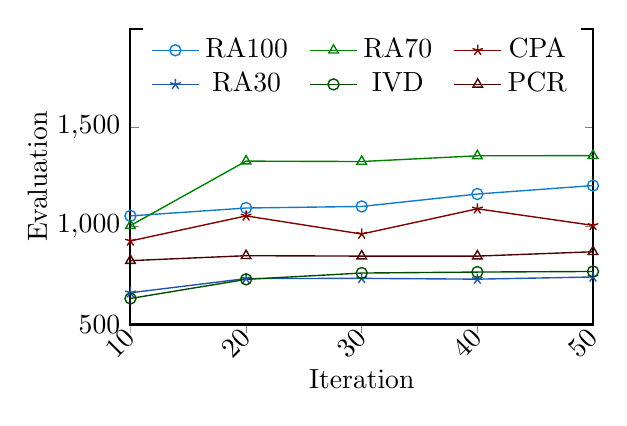
\begin{tikzpicture}
%remove space surrounding text nodes and the whole picture caused by text
%[every node/.style={inner sep=0,outer sep=0}]

%\pgfplotstableread{
%Iteration IVD\_IVD      
%1       99.69	   
%2       99.59	   
%3       99.58	  
%4       99.80	   
%5       99.85	   
%6       99.11	   
%7       87.73	   
%8       99.83	  
%9       99.42
%10      99.68
%}\loadedtable

\pgfplotstableread{
Iteration RA100 RA70	CPA	RA30	IVD	PCR
1	1051	1002	924	661	632	824
2	1091	1329	1051	733	729	849
3	1099	1327	959	734	761	847
4	1162	1356	1087	730	766	847
5	1205	1357	1003	741	769	869

}\loadedtable

\begin{axis}[
%xaxis styles
%xticklabels={s5378,s9234, s13207, s15850, s38584,systemcdes, mem\_ctrl, usb\_funct, ac97\_ctr, pci\_bridge32}, 
xticklabels={10, 20, 30, 40, 50},
xtick={1,...,5},
%x axis limits
xmin=1, xmax=5,
%x and y axes scaling
x=1.4685714cm, y=0.0025cm, 
x tick label style={rotate=45, xshift=0pt,yshift=0pt,anchor=east, 
%"inner sep" removes the space surrounding label tick texts at the bottom,
%so that there is no useless white space at the lower boundary of the picture. The
%space of tick label texts need to be removed because they are the lowest
%units without an xlable
inner sep=0}, 
xticklabel pos=left, xtick align=outside, xtick pos=left,
%
%y axis limits
ymin=500, ymax=2000, 
%yaxis styles
ylabel={Evaluation}, 
xlabel={Iteration}, 
%"inner sep" for ylabel removes the white space on the leftmost edge of the picture
ylabel style={inner sep=0}, 
ylabel shift=0pt, ytickmin=500,ytickmax=1500, 
% ytick = {700,800,900,1000,1100,1200,1300}, yticklables = {700,800,900,1000,1100,1200,1300}
%
%legend styles
legend columns=3, 
legend style={
at={(0.5,0.87)}, anchor=center, 
%column separation between legend items
/tikz/every even column/.append style={column sep=0.2cm},
%distance between legend symbols and text nodes
%column sep=2.5cm,
%space surrounding the text boxes in legend
%nodes={inner xsep=20pt},
%no stroke in legend
draw=none, 
},
%
%axis drawing line width
line width=0.75pt,
major tick length=3pt,
]  \addplot[sharp plot, line width=0.5pt, cyan!60!blue, mark=o, fill=none] table[x=Iteration,y=RA100] {\loadedtable};
\addplot[sharp plot, line width=0.5pt, green!50!black, mark=triangle, fill=none] table[x=Iteration,y=RA70] {\loadedtable};
\addplot[sharp plot, line width=0.5pt, red!50!black, mark=star, fill=none] table[x=Iteration,y=CPA] {\loadedtable};
\addplot[sharp plot, line width=0.5pt, cyan!30!blue, mark=star, fill=none] table[x=Iteration,y=RA30] {\loadedtable};
\addplot[sharp plot, line width=0.5pt, green!30!black, mark=o, fill=none] table[x=Iteration,y=IVD] {\loadedtable};
\addplot[sharp plot, line width=0.5pt, red!30!black, mark=triangle, fill=none] table[x=Iteration,y=PCR] {\loadedtable};
   %\addplot[sharp plot, line width=0.5pt, green!50!black, mark=triangle, fill=none] table[x=Iteration,y=tested] {\loadedtable};
   %\addplot[sharp plot, line width=0.5pt, red!50!black, mark=star, fill=none] table[x=Iteration,y=nobuffer] {\loadedtable};
\legend{RA100,RA70,CPA,RA30,IVD,PCR}
\end{axis}
\end{tikzpicture}

%\begin{tikzpicture}
\begin{axis}[
x=1.1cm, y=0.27cm, ymax=12, line width=0.75pt,
ylabel={Channel (Valve) Ratio}, ylabel shift=-6pt, 
xtick={1,...,6},xticklabels={RA100, RA70, CPA, RA30, IVD, PCR},
x tick label style={rotate=330, xshift=-15pt,yshift=-5pt,anchor=west}, 
xticklabel pos=left, xtick align=outside, xtick pos=left,
ytickmin=0,ytickmax=10, 
ytick={0,5,10}, yticklabels={0,0.5,1},
legend columns=2, legend style={at={(0.5,0.9)}, anchor=center, nodes={inner xsep=2pt},
draw=none, column sep=1pt},
ybar=0pt, bar width=7
]
   \addplot[line width=0.5pt, black, fill=orange!70!white] table[x=cir,y=edge] 
{edge_valve_percentage.dat};
   \addplot[line width=0.5pt, black, fill=blue!65!orange] table[x=cir,y=valve] 
{edge_valve_percentage.dat};

   \legend{Channel\hspace*{8pt}, Valve\hspace*{8pt}}
\end{axis}
\end{tikzpicture}

\caption{Average convergence curves of the proposed genetic algorithm.}
\label{fig:iteration}
}
\end{figure}

\begin{figure}[t]
    \centering
    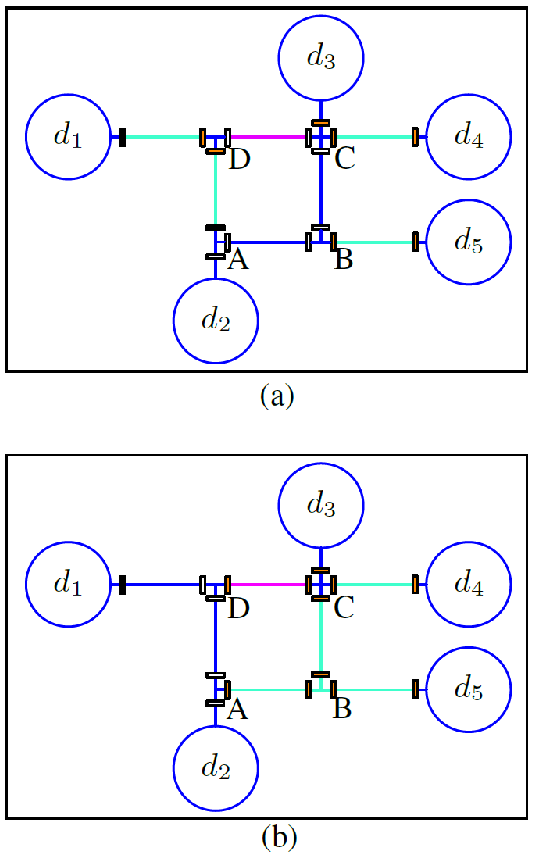
\includegraphics[width=0.6\linewidth]{Visio/RA30_exe_flow.pdf}
    %\input{Fig/RA30_exe_flow.pdf_tex}
  \caption{Snapshots of the synthesized chip executing RA30 at different times. The channel segments in blue are transporting and in purple are caching fluid samples.}
      \label{fig:RA30_exe_1}
%\vspace{-0.5cm}
\end{figure}

\begin{figure}[t]
    \centering
    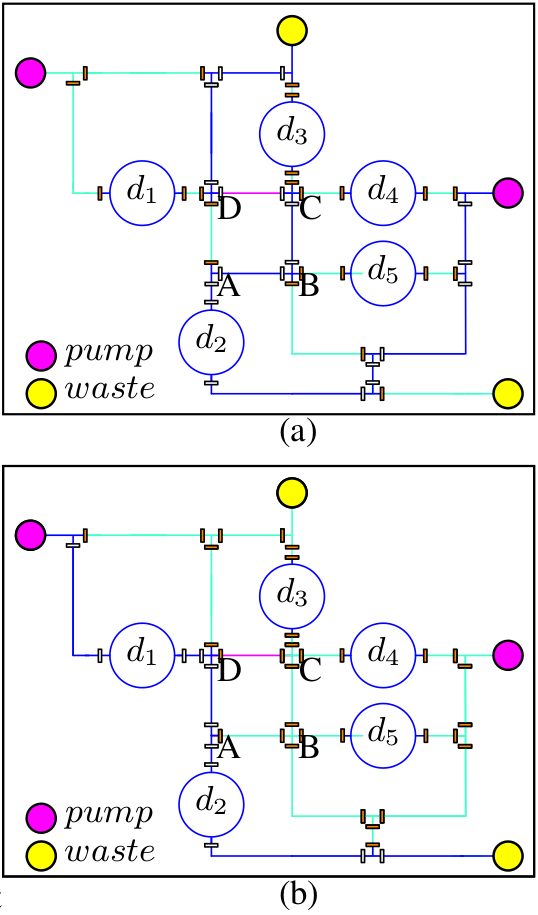
\includegraphics[width=0.7\linewidth]{Visio/RA30_exe_flow_test_ver3.png}
    %\input{Fig/RA30_exe_flow_test.pdf_tex}
  \caption{Snapshots of the synthesized chip executing RA30 with constructed flow paths at different times. The channel segments in blue are transporting and in purple are caching fluid samples.}
      \label{fig:RA30_exe_2}
%\vspace{-0.5cm}
\end{figure}

In architectural synthesis, we start with a connection grid. After synthesis, only the channels that are used at least once are kept in the result. The ratios of the number of used channels to the total number of all the channels in the grid is shown in \figname~\ref{fig:edge_valve_percentage}, where all these ratios are smaller than 1, and a half of them are even below 0.5, indicating that the architectural synthesis approach confines resource usage effectively on only a part of channels.  After removing the unused channels, the number of valves is also reduced, as shown by the valve ratios in \figname~\ref{fig:edge_valve_percentage}.

To validate the efficiency of the proposed distributed channel-storage architecture, the results of comparing execution time and number of valves for our method and the method using a dedicated storage are reported in \figname~\ref{fig:exe_time_valve_cmp}.
\textcolor{red}{The ratios are computed as ��our results/the results using dedicated storage��.}

\textcolor{red}{It can be seen from \figname~\ref{fig:exe_time_valve_cmp} that channel storage architecture leads to a relatively higher execution efficiency of bioassays, mainly due to the following reasons: 1) channel storage can be considered as distributing the storage cells of a dedicated storage to the whole chip plane in an optimized manner, leading to an ``on-the-spot" fluid store/fetch with high efficiency, 2) in the proposed method, by constructing storage channels at appropriate positions while finding optimized flow paths for fluid transportation tasks, congestion problem can be alleviated effectively, 3) when using a dedicated storage with fixed position, conflicts can also occur between store/fetch operations and fluid transportation tasks since they may share the same flow channels during their execution, and 4) the structure of a dedicated storage (see \figname~\ref{fig:valve_mixer_storage}(c) and \figname~\ref{fig:device_storage}(c)), as discussed in Section I, suffers from the drawback of bandwidth limitation.}

\textcolor{red}{Additionally, from the comparison in \figname~\ref{fig:exe_time_valve_cmp}, we can see that the number of valves used in the chip is also reduced in the channel storage architecture. This is mainly because: 1) a dedicated storage usually contains quite a number of valves inside the multiplexer-like ports as shown in \figname~\ref{fig:valve_mixer_storage}(c) and 2) although two valves should be placed at the ends of a storage channel, these valves can be saved in most cases by sharing the valves placed at channel crossings.}

\textcolor{red}{
  Moreover, in \cite{minhass2012architectural} a top-down synthesis flow is proposed to generate chip architectures with minimized application completion time. This method, however, still adopts the traditional dedicated storage to deal with the intermediate fluids generated during the execution of bioassays. To further verify the effectiveness of the proposed method and the distributed channel-storage architecture, we implemented the method in \cite{minhass2012architectural} and ran both algorithms on the same benchmarks. Table~\ref{tb_Minhass_compare} shows the comparison results, where the columns $t^{E'}$, $n_v$ and $l_n$ represent the completion time of the bioassay, the number of valves in the chip, and the total channel length.}

\textcolor{red}{
   It can be seen from Table~\ref{tb_Minhass_compare} that the proposed algorithm achieves shorter completion time of the bioassay on most test cases. There are two major reasons for these resutls: 1) dedicated storage suffers from the drawbacks of bandwidth limitation and fixed position on the chip as discussed in Section~\ref{introduction}, leading to a low efficiency of fluid store and fetch. In contrast, by caching fluids on-the-spot with distributed channel storage and coordinating the relations between fluid caching and transportation without any conflict, the efficiency of fluid store and fetch can be improved significantly and 2) in \cite{minhass2012architectural} the traditional heuristic list-scheduling method is adopted to compute a feasible scheduling scheme. The solution quality, however, is limited due to the greedy strategy adopted in the list scheduling. On the other hand, the proposed method further takes the storage optimization into account in the high-level synthesis stage to reduce the total amount of storage time, thus improving the execution efficiency of the assay. Moreover, the number of valves used in the proposed method is fewer than that of \cite{minhass2012architectural} due to the following reasons: 1) independent flow paths need to be constructed between devices and dedicated storages, leading to more channel crossings and 2) a dedicated storage also requires quite a number of valves to direct the fluid flow as can be seen from \figname~\ref{fig:valve_mixer_storage}(c). Also, the proposed method leads to an overall shorter channel length as can be seen from Table~\ref{tb_Minhass_compare}.}

In the flow-path planning stage, since the proposed genetic algorithm plays an important role in determining the new biochip architecture, to evaluate its efficiency, Fig.~\ref{fig:iteration} illustrates the corresponding convergence curves with respect to different bioassays. It can be seen that the average fitness level of the population is improved as iteration time increases, and the proposed algorithm reaches a convergence quickly in most of the test cases.
% Note that since the genetic algorithm works in a random manner, stochastic fluctuations may occur during iterations, leading to an unstable region in the convergence curve of the assay ``CPA", but our algorithm can still find a feasible flow-path planning solution for this assay.


\subsection{\textcolor{red}{Snapshots of Assay Execution}}

  Finally, We show the execution snapshots of the assay RA30
  in \figname~\ref{fig:RA30_exe_1} and \figname~\ref{fig:RA30_exe_2}, respectively.
  \figname~\ref{fig:RA30_exe_1} demonstrates the fluid transportation without considering the actual flow paths construction. In \figname~\ref{fig:RA30_exe_1}(a), a transportation path is formed as $d_2\to A\to B \to C \to D $ to store a fluid sample into the channel segment between $C$ and $D$. In \figname~\ref{fig:RA30_exe_1}(b), a transportation path is constructed as $d_1\to D \to A \to d_2$ while the channel segment between $C$ and $D$ is caching a fluid sample.
  \figname~\ref{fig:RA30_exe_2} demonstrates the fluid transportation on the chip architecture after completing the flow-path palnning. In \figname~\ref{fig:RA30_exe_2}(a), a flow path is
formed as $pump \to d_2\to A \to B \to C \to D\to waste$ to store a fluid sample
into the channel segment between $C$ and $D$. In \figname~\ref{fig:RA30_exe_2}(b), a flow path is formed as $pump
\to d_1 \to D \to A \to d_2 \to waste$, while an intermediate liquid is stored between $C$ and $D$.



